\documentclass{article}

\usepackage[main,final,nonatbib]{template/neurips_2026}
\usepackage[utf8]{inputenc}
\usepackage[T1]{fontenc}
\usepackage{hyperref}
\usepackage{url}
\usepackage{booktabs}
\usepackage{amsmath,amssymb,amsfonts}
\usepackage{microtype}
\usepackage{graphicx}
\usepackage{tabularx}
\usepackage{array}
\hypersetup{hidelinks}

\graphicspath{{../results/}}
\newcommand{\R}{\mathbb{R}}
\newcommand{\E}{\mathbb{E}}
\newcommand{\smin}{\sigma_{\min}}

\title{Conditional Flow Matching on a Two-Dimensional Checkerboard}

\author{%
  Tage Sköldefors \\
  KTH Royal Institute of Technology \\
  \And
  \textit{Second group member pending} \\
  KTH Royal Institute of Technology \\
}

\begin{document}
\maketitle

\begin{abstract}
We implement Conditional Flow Matching (CFM) with conditional optimal-transport paths and reproduce the two-dimensional checkerboard mechanism of Lipman et al.\ A neural vector field transports Gaussian noise into all eight target tiles. Increasing sampling cost from 4 to 20 neural-function evaluations reduces sliced Wasserstein distance from 0.2272 to 0.2206, with little gain beyond 8. Sweeping endpoint noise $\smin$ over three seeds gives no resolved metric difference, although $\smin=0.30$ visibly smooths tile boundaries.
\end{abstract}

\section{Algorithm and paper thesis}

\paragraph{Flow Matching.}
A continuous normalizing flow represents a time-dependent velocity field $v_\theta:[0,1]\times\R^d\to\R^d$. Starting from Gaussian noise, samples evolve by the neural ODE
\begin{equation}
  \frac{dX_t}{dt}=v_\theta(t,X_t), \qquad X_0\sim\mathcal N(0,I).
  \label{eq:ode}
\end{equation}
Solving to $t=1$ defines the model distribution \cite{chen2018}. The paper's thesis is that this model can be trained without ODE simulation by regressing velocities along fixed probability paths \cite{lipman2023}. The desired marginal velocity is intractable, but Lipman et al.\ prove that regression on tractable paths conditioned on one data sample has the same parameter gradient as the marginal Flow Matching objective.

\paragraph{Conditional OT path.}
For $Z\sim\mathcal N(0,I)$, data $X_1\sim q$, time $t\sim U[0,1]$, and $\smin\in[0,1)$, the conditional path, its derivative, and the resulting objective are
\begin{align}
  X_t &= \bigl[1-(1-\smin)t\bigr]Z+tX_1, \label{eq:path}\\
  \frac{dX_t}{dt} &= X_1-(1-\smin)Z, \label{eq:target}\\
  \mathcal L_{\mathrm{CFM}}(\theta)=
  &\E\left\|v_\theta(t,X_t)-[X_1-(1-\smin)Z]\right\|_2^2.
  \label{eq:cfm}
\end{align}
The target is constant for each sampled pair. These three lines are the mathematical training core. Each conditional trajectory is a constant-speed Gaussian OT displacement, but the induced \emph{marginal} flow need not be globally optimal \cite{lipman2023}.

\paragraph{Training and generation.}
Each iteration samples $(X_1,Z,t)$, constructs Eq.~\eqref{eq:path}, and minimizes Eq.~\eqref{eq:cfm} with Adam. Training is simulation-free; generation draws fresh noise and integrates Eq.~\eqref{eq:ode}. Our explicit midpoint rule evaluates $v_\theta$ twice per step.

\clearpage
\section{Reduced reproduction}

\subsection{Target and implementation}

We reproduce the mechanism of Figure~4 in Lipman et al., rather than their large image experiments: a Gaussian source is transported into a two-dimensional eight-tile checkerboard, and sampling is compared at low neural-function-evaluation (NFE) budgets. This isolates the probability path and numerical sampler with modest computation.

The target sampler draws $x\sim U[-2,2]$ and alternates two unit-height vertical bands according to $\lfloor x\rfloor\bmod 2$, then scales both coordinates by two. We generated 20,000 training and 5,000 held-out observations. The vector field is a multilayer perceptron taking $(t,x_1,x_2)$ and returning a two-dimensional velocity. It has three hidden layers of width 128 with SiLU activations. We train for 5,000 iterations using Adam, learning rate $2\times10^{-3}$, batch size 512, and gradient-norm clipping at 10. The baseline is $\smin=0.10$.

\begin{table}[h]
  \caption{Configuration used in the full experiment.}
  \label{tab:config}
  \centering
  \small
  \begin{tabular}{@{}ll@{\hspace{2em}}ll@{}}
    \toprule
    Setting & Value & Setting & Value \\
    \midrule
    Training samples & 20,000 & Test/generated samples & 5,000 \\
    Network & $3\times128$, SiLU & Optimizer & Adam, $2\cdot10^{-3}$ \\
    Batch/iterations & 512 / 5,000 & Seeds & 11, 22, 33 \\
    Baseline $\smin$ & 0.10 & ODE solver & Explicit midpoint \\
    SW projections & 256 & Evaluation NFE & 20 \\
    \bottomrule
  \end{tabular}
\end{table}

\paragraph{What the paper left unspecified for this reproduction.}
Figure~4 establishes the qualitative checkerboard experiment, but does not fully determine a small standalone implementation. We therefore chose the exact checkerboard coordinates, MLP depth and width, optimizer settings, training budget, held-out sample size, midpoint solver, and sliced Wasserstein (SW) evaluation protocol. These are implementation choices, not paper-reported hyperparameters. We also use Euclidean velocity MSE summed over the two coordinates and average it over the minibatch.

\begin{figure}[h]
  \centering
  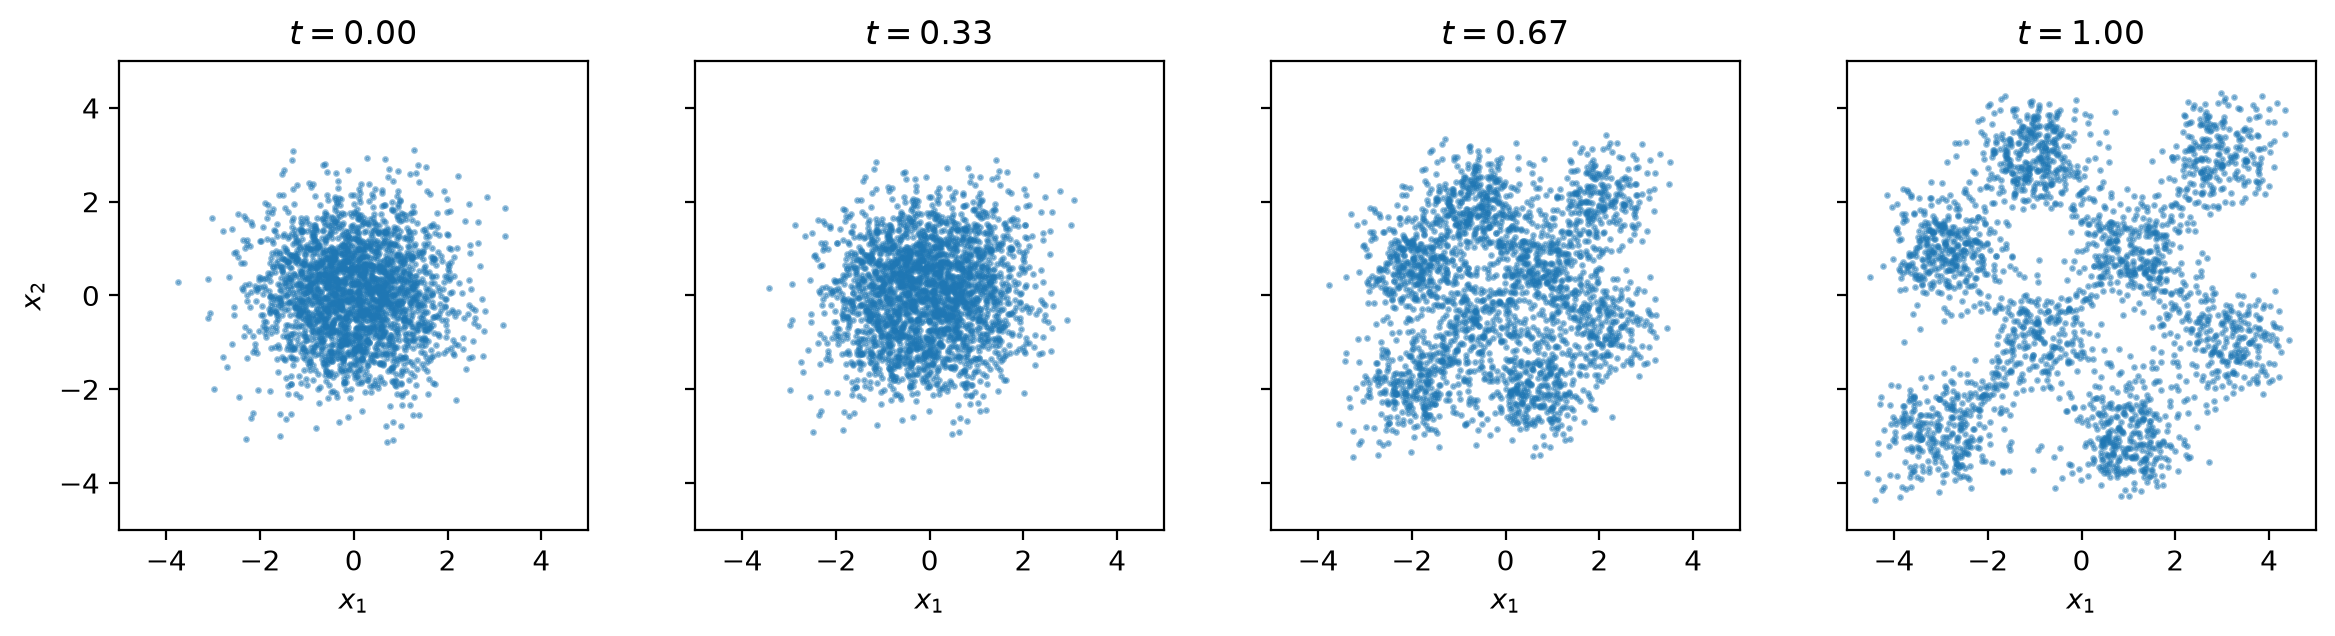
\includegraphics[width=\linewidth]{reproduction_trajectory.png}
  \caption{Learned baseline transport for seed 11. One Gaussian cloud evolves continuously into the eight checkerboard modes. The network is evaluated along a single 30-step midpoint trajectory; panels show the same particles at four times.}
  \label{fig:trajectory}
\end{figure}

Figure~\ref{fig:trajectory} shows the qualitative probability path. Structure appears by $t=2/3$, and the final cloud occupies all eight modes. Compared with the sharp uniform target tiles, the model retains rounded boundaries and some probability mass in the gaps. This is a successful reduced reproduction of the paper's central visual mechanism, but not an exact reconstruction of its unpublished toy hyperparameters.

\paragraph{Hand check.}
For $Z=(1,-2)$, $X_1=(3,1)$, $t=0.25$, and $\smin=0.1$, Eqs.~\eqref{eq:path}--\eqref{eq:target} give $X_t=(1.525,-1.3)$ and target velocity $(2.1,2.8)$. We used this calculation to check the core path and velocity formulas before running the experiment.

\clearpage
\subsection{Sampling cost}

Figure~\ref{fig:nfe} compares held-out checkerboard data with samples from the designated baseline fit (seed 11, $\smin=0.10$). Since midpoint uses two field evaluations per step, NFE 4, 8, 10, and 20 correspond to 2, 4, 5, and 10 integration steps. Every panel starts from the same Gaussian noise, so visual differences isolate numerical integration budget.

\begin{figure}[h]
  \centering
  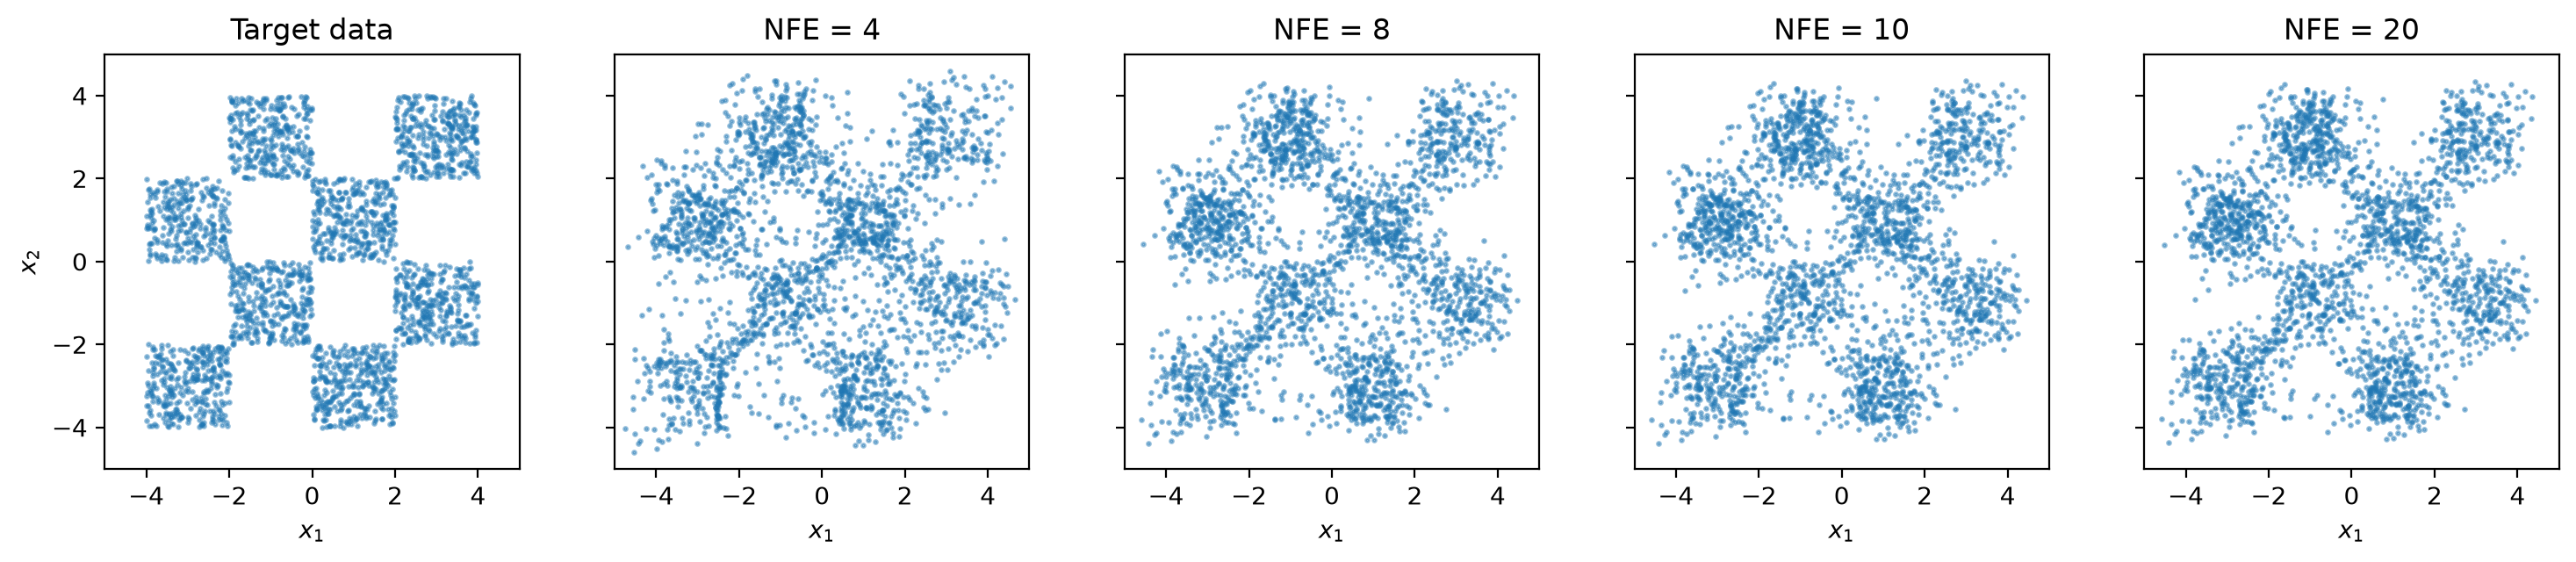
\includegraphics[width=\linewidth]{reproduction_nfe.png}
  \caption{Reduced low-cost sampling reproduction. Even NFE 4 finds all modes, while additional evaluations stabilize particle locations and slightly sharpen the geometry.}
  \label{fig:nfe}
\end{figure}

For a quantitative diagnostic, we use sliced 2-Wasserstein distance: project generated and held-out samples onto 256 random unit directions, compute exact one-dimensional empirical Wasserstein distances after sorting, and average squared discrepancies before taking a square root \cite{bonneel2015}. Lower is better.

\begin{table}[h]
  \caption{Sampling cost for the baseline seed. Differences beyond NFE 8 are small relative to the overall model error.}
  \label{tab:nfe}
  \centering
  \begin{tabular}{@{}rrrrr@{}}
    \toprule
    NFE & 4 & 8 & 10 & 20 \\
    \midrule
    Sliced Wasserstein & 0.2272 & 0.2216 & 0.2208 & 0.2206 \\
    \bottomrule
  \end{tabular}
\end{table}

The improvement from NFE 4 to 8 is $0.0056$, whereas the improvement from 8 to 20 is only $0.0010$. Thus the trained OT-path field is usable at low solver cost, matching the qualitative message of the paper. However, this table measures numerical refinement of one learned field, not an OT-versus-diffusion comparison. It therefore supports only the narrower claim that our baseline is relatively insensitive to additional midpoint steps after NFE 8.

\paragraph{Optimization behavior.}
For the baseline seed, the 100-step mean CFM loss falls rapidly from about 8.1 to below 6.9 during the first 500 iterations, then fluctuates near 6.6. A nonzero plateau is expected: the network observes $(t,X_t)$ but not the paired endpoint $X_1$ or noise $Z$, so different conditional paths can imply different velocities at similar locations. Under squared loss, the fitted marginal field averages those conditional targets.

\paragraph{Reproducibility.}
The submitted program regenerates all fits, metrics, and figures with one command. It records the full configuration and library versions. After simplifying the implementation, we repeated the complete CPU run and recovered the recorded metrics, configuration, summary, and figures exactly. Checkpoints are excluded from version control because they are regenerated by the experiment command; all report figures and CSV/JSON evidence are tracked.

\clearpage
\section{Variation: endpoint smoothing}

\paragraph{Question and protocol.}
The path ends at $X_1+\smin Z$. We vary $\smin\in\{0.01,0.10,0.30\}$ while holding all other settings fixed. We predicted a tradeoff: small $\smin$ targets sharp endpoints but may require a more accurate field; large $\smin$ may simplify regression while blurring gaps. Each value uses seeds 11, 22, and 33. Within each seed, training data, initialization, test data, metric projections, and initial sampling noise are paired across $\smin$.

\begin{table}[h]
  \caption{Variation results at NFE 20. Values are mean $\pm$ sample standard deviation over three paired seeds.}
  \label{tab:variation}
  \centering
  \begin{tabular}{@{}ccc@{}}
    \toprule
    $\smin$ & Sliced Wasserstein & Final CFM loss \\
    \midrule
    0.01 & $0.1573\pm0.0568$ & $6.7757\pm0.0317$ \\
    0.10 & $0.1494\pm0.0637$ & $6.5949\pm0.0305$ \\
    0.30 & $0.1556\pm0.0628$ & $6.2378\pm0.0280$ \\
    \bottomrule
  \end{tabular}
\end{table}

\begin{figure}[h]
  \centering
  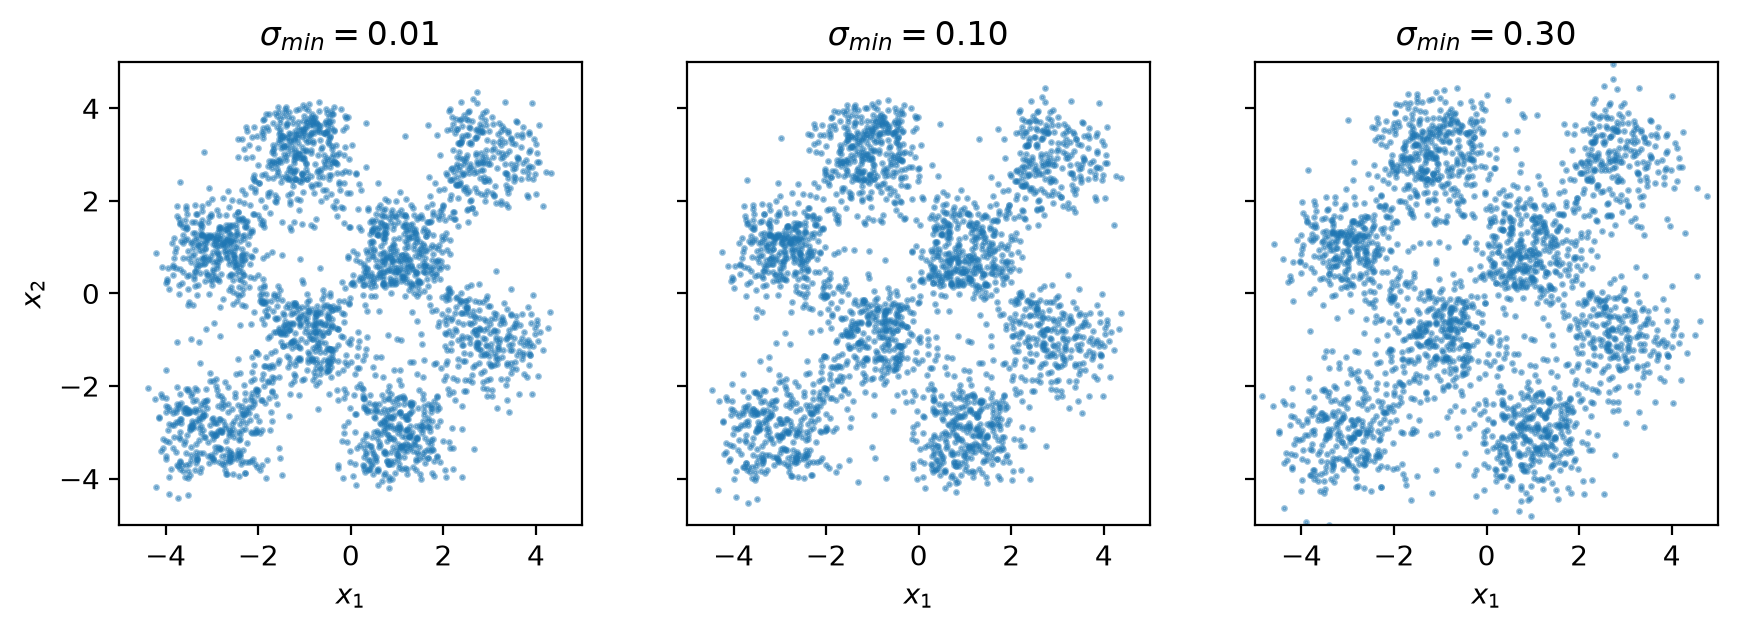
\includegraphics[width=0.94\linewidth]{variation_samples.png}
  \caption{Paired-noise samples for seed 11 at NFE 20. Larger $\smin$ visibly diffuses tile boundaries and leaves more mass in the gaps, but all settings recover the same modal layout.}
  \label{fig:variation}
\end{figure}

\paragraph{Result.}
Training loss decreases monotonically with $\smin$, but Eq.~\eqref{eq:target} shows that larger $\smin$ reduces the target's noise term and changes the endpoint; this is not evidence of better samples. Mean SW distances differ by at most 0.0079, versus across-seed standard deviations of 0.057--0.064. Thus no tested value reliably improves the metric. Figure~\ref{fig:variation} still supports the predicted mechanism: $\smin=0.30$ gives less compact tiles and more between-mode mass. Smoothing is visible, but this metric and three-seed experiment do not resolve a monotone quality tradeoff.

\paragraph{Limitations.}
Three seeds give weak uncertainty estimates, and seed 11 is worse in every setting. Sliced Wasserstein emphasizes global projections and may miss local leakage into checkerboard gaps; an off-support-mass metric and more paired seeds would test the visual effect more directly. The study also uses one toy distribution and does not compare diffusion paths, solvers, or capacities.

\section{Conclusion}

We implemented CFM without a Flow Matching library and reproduced checkerboard transport and low-NFE sampling. Training needs sampled regression pairs; generation integrates the learned field. Stronger endpoint smoothing is visible and lowers training loss, but does not reliably change sliced Wasserstein distance. The next test should add an off-support metric and more paired seeds.

\clearpage
\begin{thebibliography}{9}

\bibitem{lipman2023}
Yaron Lipman, Ricky T. Q. Chen, Heli Ben-Hamu, Maximilian Nickel, and Matt Le.
\newblock Flow Matching for Generative Modeling.
\newblock In \emph{International Conference on Learning Representations}, 2023.
\newblock \url{https://openreview.net/forum?id=PqvMRDCJT9t}.

\bibitem{chen2018}
Ricky T. Q. Chen, Yulia Rubanova, Jesse Bettencourt, and David Duvenaud.
\newblock Neural Ordinary Differential Equations.
\newblock In \emph{Advances in Neural Information Processing Systems 31}, 2018.

\bibitem{bonneel2015}
Nicolas Bonneel, Julien Rabin, Gabriel Peyr\'e, and Hanspeter Pfister.
\newblock Sliced and Radon Wasserstein Barycenters of Measures.
\newblock \emph{Journal of Mathematical Imaging and Vision}, 51(1):22--45, 2015.

\end{thebibliography}

\clearpage
\section*{AI-use statement}

\noindent\textbf{Review before signing.} This report was prepared with AI assistance. Both group members must independently verify every equation, rerun and understand the code, revise the analysis into their own substantiated account, and ensure the disclosure below is complete. Do not sign until every declaration is true.

\subsection*{1. Tools used}

\begin{tabularx}{\linewidth}{@{}p{0.34\linewidth}X@{}}
  \toprule
  Tool and version & Used for \\
  \midrule
  OpenAI Codex, GPT-5 family (accessed 2026-09-22) & Reference implementation, debugging, experiment orchestration, mathematical checking, literature summary, LaTeX drafting, and layout verification. \\
  \bottomrule
\end{tabularx}

\subsection*{2. Where it was used}

\begin{tabularx}{\linewidth}{@{}p{0.43\linewidth}X@{}}
  \toprule
  Category & Description \\
  \midrule
  $\boxtimes$ Writing or debugging code & Drafted the compact three-module reference implementation, plotting, metrics, and experiment runner; assisted with debugging and reproducibility. \\
  $\boxtimes$ Deriving or checking mathematics & Checked the conditional OT interpolation, its derivative, the CFM objective, and the midpoint update. \\
  $\boxtimes$ Finding or summarizing background literature & Located and summarized the Flow Matching, neural ODE, and sliced Wasserstein sources. \\
  $\boxtimes$ Other & Drafted and formatted this report from program-generated results and assisted with result interpretation. \\
  \bottomrule
\end{tabularx}

\subsection*{3. Declaration}

We declare that:
\begin{itemize}
  \item every number, figure and table in this report was produced by running our own submitted code;
  \item we understand every line of that code and can explain, modify and extend it without assistance;
  \item the substance of this work -- the implementation, experiment, analysis and writing -- is our own, and is not AI-generated work that we revised;
  \item the account given above is complete and accurate.
\end{itemize}
We understand that non-disclosure, or presenting AI-generated work as our own, is academic misconduct and will be reported.

\subsection*{4. Contributions}

\begin{tabularx}{\linewidth}{@{}p{0.20\linewidth}p{0.13\linewidth}X p{0.18\linewidth}@{}}
  \toprule
  Name & KTH ID & Contribution & Signature \\
  \midrule
  Tage Sköldefors & \rule{0.9\linewidth}{0.4pt} & \rule{\linewidth}{0.4pt} & \\
  \addlinespace[1.2em]
  \rule{\linewidth}{0.4pt} & \rule{0.9\linewidth}{0.4pt} & \rule{\linewidth}{0.4pt} & \\
  \addlinespace[1.2em]
  \bottomrule
\end{tabularx}

\vspace{1.5em}
\noindent Place and date: \hrulefill

\end{document}
